% !TEX program = pdflatex
\documentclass[letterpaper, 10pt, conference]{IEEEtran}

\usepackage{amsmath,amssymb,amsfonts}
\usepackage{algorithmic}
\usepackage{algorithm}
\usepackage{graphicx}
\usepackage{textcomp}
\usepackage{booktabs}
\usepackage{multirow}
\usepackage{cite}
\usepackage{hyperref}
\usepackage{xcolor}
\usepackage{bm}

% Compact lists
\usepackage{enumitem}
\setlist{nosep}

% Math shortcuts
\newcommand{\R}{\mathbb{R}}
\newcommand{\balpha}{\bm{\alpha}}
\newcommand{\bt}{\bm{t}}
\newcommand{\bx}{\bm{x}}
\newcommand{\bu}{\bm{u}}
\newcommand{\by}{\bm{y}}
\newcommand{\bz}{\bm{z}}
\newcommand{\bK}{\bm{K}}

\begin{document}

\title{TinyMPC with Differential Flatness:\\
  $\alpha$-Parameterized Templates for Efficient Quadrotor Control}

\author{
  \IEEEauthorblockN{Jianghan Zhang}
  \IEEEauthorblockA{Dartmouth College\\
  \texttt{jianghan.zhang.gr@dartmouth.edu}}
}

\maketitle

% ================================================================
\begin{abstract}
TinyMPC enables real-time model-predictive control on microcontrollers
by caching the infinite-horizon Riccati solution and requiring
only matrix--vector products at each ADMM iteration.
However, its linearization is fixed at a single operating point
(typically hover), which degrades tracking performance for aggressive
trajectories.
We exploit the \emph{differential flatness} of quadrotor dynamics
to reparameterize the linearization by a flat parameter
$\balpha = (a_x, a_y, a_z, \psi)$.
This yields closed-form equilibria and Jacobians---no automatic
differentiation required---making the computation FPGA-portable.
We present three extensions of TinyMPC:
(i)~\emph{Flat Template MPC}, which precomputes DARE caches at a grid
of $\balpha$ values for online nearest-neighbor lookup;
(ii)~\emph{Analytic Template}, a zero-iteration state-feedback
controller using first-order gain interpolation (${\sim}260$
arithmetic operations per control output);
and (iii)~\emph{Barrier-Augmented Template}, which absorbs
log-barrier constraint information into the DARE cache so
that the zero-iteration controller is inherently constraint-aware,
with optional Newton--IPM refinement at quadratic convergence.
Preliminary Python simulations on a Crazyflie-scale quadrotor show
that, on figure-eight trajectory tracking,
the Flat Template achieves tracking accuracy within 6\% of
online relinearization ($0.035$\,m average position error)
at $29\times$ lower wall-clock time,
while the Analytic Template maintains $0.036$\,m error with
zero ADMM iterations.
\end{abstract}

% ================================================================
\section{Introduction}\label{sec:intro}

Model-predictive control (MPC) is a powerful framework for controlling
highly dynamic robots subject to state and input constraints~\cite{tinympc}.
TinyMPC~\cite{tinympc} demonstrated that, by caching the
infinite-horizon discrete algebraic Riccati equation (DARE) solution
offline and performing only matrix--vector products online,
the ADMM-based MPC solver can run on microcontrollers with as little
as 192\,kB of RAM at rates exceeding 500\,Hz.

A key assumption in TinyMPC is that the dynamics are linearized
at a \emph{fixed operating point}---typically the hover equilibrium
for a quadrotor.
This is reasonable for near-hover regulation but becomes a limitation
for aggressive trajectory tracking, where the true linearization
varies significantly along the reference.
The standard remedy---online relinearization at each timestep---requires
Jacobian evaluation (via automatic differentiation or finite differences)
and a fresh DARE solve, both of which are computationally expensive
and ill-suited for resource-constrained platforms.

We observe that quadrotor dynamics are \emph{differentially flat}
with flat output $\by = (p_x, p_y, p_z, \psi)$~\cite{mellinger2011,murray1995}.
This classical property has been widely used for trajectory
generation~\cite{mellinger2011,mueller2015}, but its implications
for \emph{MPC solver structure} have received less attention.
We show that flatness enables a closed-form parameterization of
both the equilibrium and the Jacobian by a single four-dimensional
\emph{flat parameter}
$\balpha = (a_x, a_y, a_z, \psi) \in \R^4$,
representing the commanded translational acceleration and yaw angle.
Because the resulting expressions involve only elementary trigonometric
and algebraic operations, they require no automatic differentiation
and are directly implementable on FPGAs.

Crucially, because $\balpha$ is four-dimensional---compared to the
$n=12$ dimensional state---it serves as a natural
\emph{scheduling variable} for the DARE solution.
This connects our approach to classical gain scheduling~\cite{rugh2000}
and linear parameter-varying (LPV) control~\cite{shamma1991},
but with the scheduling space compressed from $\R^n$ to $\R^4$
by the flat map.
We make this connection precise in Section~\ref{sec:analytic}
and show that the Analytic Template is equivalent to
a first-order gain schedule over $\balpha$, where the gain
sensitivity is obtained from perturbation analysis of the
DARE~\cite{hewer1971,konstantinov1993}.

Building on this observation, we propose three extensions of TinyMPC:

\begin{enumerate}
  \item \textbf{Flat Template MPC} (Section~\ref{sec:flat_template}):
    Precompute DARE caches at a grid of $\balpha$ values offline.
    Online, look up the nearest cache and run $K_{\mathrm{ADMM}}$
    ADMM iterations as in standard TinyMPC, but with
    $\balpha$-specific
    matrices $(A_d, B_d, K_\infty, P_\infty, C_1, C_2)$.
  \item \textbf{Analytic Template} (Section~\ref{sec:analytic}):
    Precompute the gain $K_0$ at hover and its four partial
    derivatives $\partial K / \partial \alpha_i$ offline.
    Online, interpolate $K(\balpha) \approx K_0 + \sum_i \delta\alpha_i \, \partial_i K$
    and apply a single feedback step---no ADMM iterations, no constraint
    projection.
    The total cost is ${\sim}260$ multiply-accumulate (MAC) operations.
  \item \textbf{Barrier-Augmented Template} (Section~\ref{sec:barrier}):
    Absorb log-barrier constraint penalties into the DARE cache,
    so that the zero-iteration controller inherently avoids
    actuator limits.
    Optional Newton--IPM refinement online yields hard constraint
    satisfaction at quadratic convergence.
\end{enumerate}

All flat-parameterized variants shift the coordinate frame to
the flat equilibrium $(x^*(\balpha), u^*(\balpha))$,
so the solver always operates in a neighborhood of zero
error---regardless of the trajectory aggressiveness.
Fig.~\ref{fig:hierarchy} illustrates the pipeline.

\begin{figure}[t]
  \centering
  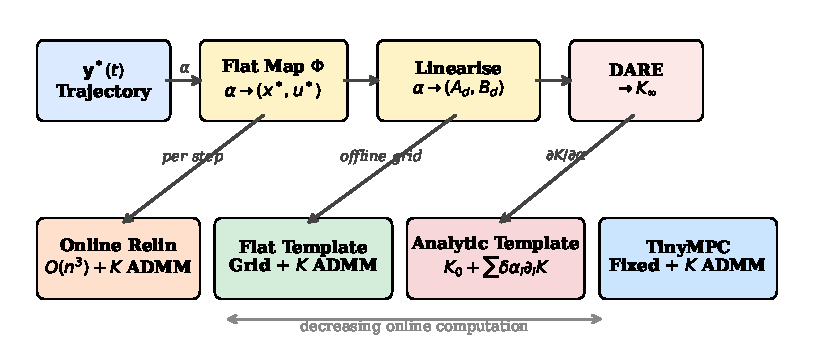
\includegraphics[width=\columnwidth]{figures/fig_hierarchy.pdf}
  \caption{Controller hierarchy.
    The flat map $\Phi$ and analytic linearization (yellow) are shared
    by all flat-parameterized variants.
    Moving right trades online computation for approximation:
    Online Relinearization re-solves DARE per step;
    Flat Template looks up a precomputed cache;
    the Analytic Template interpolates $K(\balpha)$ in ${\sim}260$ ops.}
  \label{fig:hierarchy}
\end{figure}

\subsection*{Contributions}
\begin{itemize}
  \item An explicit, autograd-free linearization of quadrotor
    dynamics parameterized by $\balpha \in \R^4$
    (Section~\ref{sec:linearize}).
  \item Flat Template MPC: an $\balpha$-indexed cache family for
    TinyMPC's ADMM solver (Section~\ref{sec:flat_template}).
  \item Analytic Template: a zero-iteration controller with
    first-order gain approximation (Section~\ref{sec:analytic}).
  \item Barrier-Augmented Template: absorbing log-barrier constraint
    information into the DARE cache for zero-iteration
    constraint-aware control, with optional IPM refinement
    at quadratic convergence (Section~\ref{sec:barrier}).
  \item Preliminary numerical validation comparing four controller
    variants on hover and figure-eight tracking
    (Section~\ref{sec:experiments}).
\end{itemize}

% ================================================================
\section{Background}\label{sec:background}

\subsection{Mathematical Preliminaries}\label{sec:prelim}

This section introduces the three mathematical tools that
the paper builds on: ADMM, the discrete algebraic Riccati
equation, and the log-barrier interior-point method.
Readers familiar with these topics may skip to
Section~\ref{sec:tinympc_background}.

\textbf{ADMM (Alternating Direction Method of Multipliers).}
Many MPC problems take the form
\begin{equation}\label{eq:admm_generic}
  \min_{z} \; f(z) \quad \text{s.t.} \quad z \in \mathcal{C},
\end{equation}
where $f$ is a smooth (often quadratic) cost and $\mathcal{C}$
encodes constraints (e.g., actuator limits, state bounds).
ADMM~\cite{boyd2011} splits this into two alternating steps
by introducing an auxiliary variable $\tilde{z}$ and a dual
variable $\lambda$:
\begin{enumerate}[label=(\alph*)]
  \item \emph{Minimize} $f$ without constraints (smooth, often
    admits a closed-form or Riccati-based solution):
    $z^{k+1} = \arg\min_z \; f(z) + \tfrac{\rho}{2}\|z - \tilde{z}^k + \lambda^k\|^2$.
  \item \emph{Project} onto constraints (often a simple clipping
    operation):
    $\tilde{z}^{k+1} = \mathrm{proj}_{\mathcal{C}}(z^{k+1} + \lambda^k)$.
  \item \emph{Update} the dual variable:
    $\lambda^{k+1} = \lambda^k + z^{k+1} - \tilde{z}^{k+1}$.
\end{enumerate}
The penalty $\rho > 0$ controls the coupling strength between
the smooth and constraint steps.
ADMM converges at a \emph{linear} rate: the primal residual
$\|z - \tilde{z}\|$ decreases geometrically with the number
of iterations~\cite{boyd2011}.
For MPC, the key property is that step~(a) has the structure
of an unconstrained LQR problem, solvable by a Riccati
recursion, while step~(b) is a componentwise clipping
operation.
This separation is what enables the DARE-caching strategy
of TinyMPC.

\textbf{Discrete Algebraic Riccati Equation (DARE).}
Consider the infinite-horizon LQR problem for the linear
system $x_{k+1} = A x_k + B u_k$ with stage cost
$\ell(x,u) = \frac{1}{2}(x^\top Q x + u^\top R u)$,
where $Q \succeq 0$ and $R \succ 0$.
The optimal cost-to-go from state $x$ is
$V^*(x) = \frac{1}{2} x^\top P x$,
where $P$ satisfies the DARE:
\begin{equation}\label{eq:dare_background}
  P = Q + A^\top P A
  - A^\top P B (R + B^\top P B)^{-1} B^\top P A.
\end{equation}
The optimal feedback gain is
$K = (R + B^\top P B)^{-1} B^\top P A$,
so that $u^* = -K x$ minimizes the infinite-horizon cost.
The closed-loop matrix $A_{\mathrm{cl}} = A - BK$ is stable:
all eigenvalues lie strictly inside the unit circle,
guaranteeing exponential convergence
$\|x_k\| \leq c \, \rho(A_{\mathrm{cl}})^k \|x_0\|$
where $\rho(A_{\mathrm{cl}}) < 1$ is the spectral radius.

The DARE is solved offline by iterating the Riccati recursion
$P_{k} = Q + A^\top P_{k+1} A - A^\top P_{k+1} B
(R + B^\top P_{k+1} B)^{-1} B^\top P_{k+1} A$
backward from a terminal condition $P_N$ until convergence.
The converged $P$ and $K$ encode the entire infinite-horizon
optimal controller in two matrices.

\textbf{Log-Barrier Interior-Point Method.}
To handle inequality constraints
$g_j(u) \leq 0$, $j = 1, \ldots, p$,
the log-barrier method~\cite{boyd2004} replaces them with
a smooth penalty:
\begin{equation}\label{eq:barrier_background}
  \min_u \; f(u) - \mu \sum_{j=1}^{p} \log(-g_j(u)),
\end{equation}
where $\mu > 0$ is the barrier parameter.
The logarithmic term is finite only when all constraints
are strictly satisfied ($g_j < 0$), and tends to $+\infty$
as any constraint approaches its boundary ($g_j \to 0^-$).
As $\mu \to 0$, the solution of~\eqref{eq:barrier_background}
approaches the solution of the original constrained problem.

For box constraints $u_{\min} \leq u \leq u_{\max}$,
$g_j(u) = u_j - u_{\max,j}$ and
$g_{j+m}(u) = u_{\min,j} - u_j$,
giving the barrier
$-\mu[\log(u_j - u_{\min,j}) + \log(u_{\max,j} - u_j)]$.
The Hessian (second derivative) of this barrier is a
diagonal matrix whose entries are large near the constraint
boundaries and small far from them.

Each subproblem~\eqref{eq:barrier_background} is smooth
and unconstrained (in the strict interior), so it can be
solved by Newton's method.
Newton's method converges \emph{quadratically}:
the error decreases as $\|e_{k+1}\| \leq C \|e_k\|^2$,
meaning that 2--3 iterations typically reduce a moderate
initial error to machine precision~\cite{boyd2004}.
This is in contrast to ADMM's linear
convergence, where a fixed fraction of the error is removed
per iteration.

\subsection{Related Work}\label{sec:related}

\textbf{Gain scheduling.}
The classical approach to controlling nonlinear systems around
varying operating points is gain scheduling~\cite{rugh2000}:
solve the linear control problem (e.g., LQR or $H_\infty$) at
a grid of operating points offline, then interpolate the resulting
gains online.
Rugh and Shamma~\cite{rugh2000} survey the extensive theory,
including conditions under which interpolated controllers
inherit stability from the frozen-parameter designs.
Our Flat Template MPC is a gain-scheduled ADMM-MPC controller
where the scheduling variable is the flat parameter $\balpha$,
and our Analytic Template is a first-order gain schedule with
an explicit interpolation formula~\eqref{eq:K_interp}.

\textbf{LPV control.}
Linear parameter-varying (LPV) systems generalize gain scheduling
by treating the varying linearization as a parameter-dependent
plant $\dot{x} = A(\theta) x + B(\theta) u$ where $\theta(t)$
is measurable in real time~\cite{shamma1991}.
Our framework fits this structure with $\theta = \balpha$,
but we exploit flatness to guarantee that $\balpha$ is a
\emph{four-dimensional sufficient statistic} for the
equilibrium---rather than requiring the full $n$-dimensional
state as scheduling variable.

\textbf{Riccati sensitivity analysis.}
The dependence of the DARE solution on system parameters has been
studied since Hewer~\cite{hewer1971}, with explicit perturbation
bounds developed by Konstantinov et al.~\cite{konstantinov1993}.
Our gain sensitivities $\partial K / \partial \alpha_i$
in~\eqref{eq:dK} are a numerical instance of this theory,
approximated by central differences.
The key practical insight is that for quadrotor dynamics,
$K(\balpha)$ varies smoothly and slowly with $\balpha$,
so a first-order expansion suffices (4\% mean relative error
over the tested range).

\textbf{Flatness-based tracking control.}
Differential flatness has been widely used for quadrotor
trajectory generation~\cite{mellinger2011,mueller2015} and
feedforward computation~\cite{faessler2018}.
Mellinger and Kumar~\cite{mellinger2011} use the flat map to
compute reference states and inputs, then track with a fixed-gain
controller.
Our approach extends this by additionally using the flat map
to parameterize the \emph{feedback gain itself},
adapting $K$ to the current operating condition through
the DARE sensitivity.

\textbf{Explicit MPC.}
An alternative to online optimization is explicit MPC~\cite{bemporad2002},
which precomputes the optimal control law as a piecewise-affine
function of the state via multi-parametric programming.
The Flat Template MPC shares the ``precompute offline, look up online''
philosophy, but avoids the exponential complexity of explicit MPC
by storing only DARE caches (not full polyhedral partitions)
and running a small number of ADMM iterations online.

\subsection{TinyMPC}\label{sec:tinympc_background}

TinyMPC~\cite{tinympc} solves the constrained linear MPC problem,
formulated as a quadratic program (QP)~\cite{osqp,boyd2011},
\begin{align}
  \min_{x_{1:N}, u_{1:N-1}} \;\;
  & \tfrac{1}{2} x_N^\top Q_f x_N
    + \sum_{k=1}^{N-1} \bigl(
      \tfrac{1}{2} x_k^\top Q x_k
      + \tfrac{1}{2} u_k^\top R u_k \bigr) \notag \\
  \text{s.t.} \;\;
  & x_{k+1} = A x_k + B u_k, \notag \\
  & x_k \in \mathcal{X},\;\; u_k \in \mathcal{U},
  \label{eq:mpc}
\end{align}
via ADMM, where $\rho > 0$ is the ADMM penalty parameter.
The key insight is that, for a sufficiently long horizon $N$,
the backward Riccati recursion converges to a steady-state
solution $(K_\infty, P_\infty)$.
The matrix $P_\infty$ is the infinite-horizon optimal
cost-to-go: it compresses the effect of all future stages
into a single $n \times n$ matrix, so that
$\frac{1}{2} \delta x^\top P_\infty \, \delta x$ approximates
the minimum cost from state $\delta x$ to the origin
over an infinite horizon.
TinyMPC solves the discrete algebraic Riccati equation (DARE)
for $P_\infty$ \emph{offline} and caches the derived quantities:
\begin{align}
  K_\infty &= (R_\rho + B^\top P_\infty B)^{-1} B^\top P_\infty A, \label{eq:kinf} \\
  C_1      &= (R_\rho + B^\top P_\infty B)^{-1}, \notag \\
  C_2      &= (A - B K_\infty)^\top, \notag
\end{align}
where $R_\rho = R + \rho I$ is the ADMM-augmented input cost
and $Q_\rho = Q + \rho I$ is the ADMM-augmented state cost.
The gain $K_\infty$ is the optimal LQR gain for the augmented
problem; $C_1$ and $C_2$ are auxiliary matrices that eliminate
all matrix inversions from the online computation.
Each ADMM iteration then requires only matrix--vector products:
\begin{enumerate}[label=(\roman*)]
  \item \emph{Backward pass}: compute feedforward corrections
    $d_k = C_1(B^\top p_{k+1} + r_k)$,
    $p_k = q_k + C_2 \, p_{k+1} - K_\infty^\top r_k$.
  \item \emph{Forward pass}: $u_k = -K_\infty x_k - d_k$,
    $x_{k+1} = A x_k + B u_k$.
  \item \emph{Slack update}: project onto constraints.
  \item \emph{Dual update}: gradient ascent on multipliers.
\end{enumerate}

The entire online computation is \emph{matrix-inversion free}.
However, the matrices $A, B$ (and hence all cached quantities)
are fixed at a single linearization point.

\subsection{Differential Flatness of Quadrotor Dynamics}\label{sec:flatness}

A quadrotor with state
$(p, \dot{p}, R, \omega) \in \R^3 \times \R^3 \times \mathrm{SO}(3) \times \R^3$
and collective thrust $T$ along the body $z$-axis satisfies
\begin{equation}\label{eq:trans}
  m \ddot{p} = T R e_3 - m g e_3.
\end{equation}
The system is differentially flat with flat output
$\by = (p_x, p_y, p_z, \psi)$~\cite{mellinger2011,murray1995}.
This means that every state and input can be expressed as an
algebraic function of $\by$ and a finite number of its time derivatives.

The flat map proceeds as follows.
Define the \emph{total acceleration vector}
\begin{equation}\label{eq:tvec}
  \bt = \ddot{p} + g e_3 = \begin{pmatrix} a_x \\ a_y \\ a_z + g \end{pmatrix},
\end{equation}
where $(a_x, a_y, a_z)$ is the commanded translational acceleration
in the world frame.
Then:
\begin{enumerate}
  \item \textbf{Thrust:} $T = m \| \bt \|$.
  \item \textbf{Attitude:} The body $z$-axis is
    $z_B = \bt / \|\bt\|$.
    Given yaw $\psi$, the rotation $R$ is fully determined.
    In Euler angles (ZYX convention):
    \begin{align}
      \phi^* &= \arcsin\!\bigl(
        (a_x \sin\psi - a_y \cos\psi) / \|\bt\| \bigr), \label{eq:phi_eq} \\
      \theta^* &= \arctan2\!\bigl(
        a_x \cos\psi + a_y \sin\psi, \; a_z + g \bigr). \label{eq:theta_eq}
    \end{align}
  \item \textbf{Angular velocity and torques:}
    determined by $p^{(3)}$ and $p^{(4)}$ (jerk and snap) through the
    kinematic and Euler equations; at equilibrium, $\omega^* = 0$.
\end{enumerate}

We define the \emph{flat parameter}
$\balpha = (a_x, a_y, a_z, \psi) \in \R^4$,
which fully specifies the equilibrium state and input:
\begin{equation}\label{eq:eq_map}
  \Phi: \balpha \;\mapsto\; (x^*(\balpha),\; u^*(\balpha)).
\end{equation}

% ================================================================
\section{Method}\label{sec:method}

\subsection{Analytic Linearization}\label{sec:linearize}

Given $\balpha$, we construct the continuous-time Jacobians
$A_c(\balpha), B_c(\balpha)$ of the 12-dimensional
Euler-angle state
$x = (p, \phi, \theta, \psi, v, \omega)$
about the flat equilibrium~\eqref{eq:eq_map}.

The $12 \times 12$ matrix $A_c$ has the block structure
\begin{equation}\label{eq:Ac}
  A_c = \begin{pmatrix}
    0_{3\times3} & 0_{3\times3} & I_3 & 0_{3\times3} \\
    0_{3\times3} & 0_{3\times3} & 0_{3\times3} & W(\phi^*,\theta^*) \\
    0_{3\times3} & G(\balpha)   & 0_{3\times3} & 0_{3\times3} \\
    0_{3\times3} & 0_{3\times3} & 0_{3\times3} & 0_{3\times3}
  \end{pmatrix},
\end{equation}
where $G(\balpha) \in \R^{3\times3}$ is the gravity coupling matrix
(derivative of the thrust vector with respect to attitude at equilibrium)
and $W(\phi^*, \theta^*)$ is the Euler-angle kinematic map
relating body angular velocity to Euler rates.

The $12 \times 4$ input matrix $B_c$ maps the four motor
thrusts to state derivatives.
It has nonzero blocks in
the velocity rows (thrust direction $\times k_t / m$,
where $k_t$ is the per-motor thrust coefficient and
$m$ is the quadrotor mass)
and the angular velocity rows
($J^{-1} M_{\mathrm{mix}}$,
where $J \in \R^{3\times3}$ is the body-frame inertia
tensor and $M_{\mathrm{mix}} \in \R^{3\times4}$ is
the motor mixing matrix that maps individual motor
thrusts to body torques via the arm geometry).

Discretization via forward Euler yields
\begin{equation}\label{eq:disc}
  A_d = I_{12} + A_c \Delta t, \qquad
  B_d = B_c \Delta t.
\end{equation}

The entire computation is closed-form trigonometry and linear algebra,
requiring no automatic differentiation.

\subsection{Flat Template MPC}\label{sec:flat_template}

Flat Template MPC extends TinyMPC by maintaining a \emph{family}
of DARE caches indexed by $\balpha$.

\textbf{Offline.}
Select a grid $\{\balpha^{(j)}\}_{j=1}^M$
(e.g., sampled along the reference trajectory).
For each grid point:
\begin{enumerate}
  \item Compute $(A_d^{(j)}, B_d^{(j)}) = \texttt{linearise}(\balpha^{(j)})$.
  \item Solve the standard (non-augmented) discrete LQR
    to obtain the terminal cost matrix $P_{\mathrm{lqr}}^{(j)}$.
  \item Solve augmented DARE~\eqref{eq:kinf} to obtain
    $K_\infty^{(j)}, P_\infty^{(j)}, C_1^{(j)}, C_2^{(j)}$.
  \item Store the full cache
    $\{A_d, B_d, K_\infty, P_\infty, C_1, C_2\}^{(j)}$.
\end{enumerate}

\textbf{Online.}
At each control step with current flat parameter $\balpha$:
\begin{enumerate}
  \item Look up the nearest cache entry
    $j^* = \arg\min_j \|\balpha - \balpha^{(j)}\|$.
  \item Compute the flat equilibrium
    $(x^*, u^*) = \Phi(\balpha)$.
  \item Form the error state $\delta x = x - x^*$.
  \item Run $K_{\mathrm{ADMM}}$ ADMM iterations using cache $j^*$
    (identical to TinyMPC's backward/forward/slack/dual passes).
  \item Apply $u = u^* + \delta u_0$, where $\delta u_0$ is
    the first-step control from the ADMM solution.
\end{enumerate}

This preserves TinyMPC's matrix-inversion-free online structure
while adapting the linearization to the current operating point.
The offline cost is $M$ DARE solves (each ${\sim}5000$ Riccati
iterations), and the online lookup is $O(M)$ nearest-neighbor search.

\subsection{Analytic Template}\label{sec:analytic}

The Analytic Template eliminates ADMM iterations entirely,
producing a control output in ${\sim}260$ arithmetic operations.

\textbf{Offline.}
\begin{enumerate}
  \item Set $\balpha_0 = (0, 0, 0, 0)$ (hover).
  \item Solve the augmented DARE at $\balpha_0$ to obtain
    the base gain $K_0 \in \R^{4 \times 12}$.
  \item For $i = 1, \ldots, 4$, compute gain sensitivities
    via central differences:
    \begin{equation}\label{eq:dK}
      \frac{\partial K}{\partial \alpha_i} \approx
      \frac{K(\balpha_0 + \epsilon \, e_i) - K(\balpha_0 - \epsilon \, e_i)}
           {2\epsilon}.
    \end{equation}
  \item Store $K_0$ and $\{\partial_i K\}_{i=1}^4$:
    a total of $5 \times 4 \times 12 = 240$ floating-point numbers.
\end{enumerate}

\textbf{Online.}
Given state $x$ and flat parameter $\balpha$:
\begin{enumerate}
  \item $\delta \balpha = \balpha - \balpha_0$.
  \item Compute $(x^*, u^*) = \Phi(\balpha)$.
  \item Interpolate the gain (192 multiply-accumulate operations):
    \begin{equation}\label{eq:K_interp}
      K(\balpha) \approx K_0 + \sum_{i=1}^{4} \delta\alpha_i \; \frac{\partial K}{\partial \alpha_i}.
    \end{equation}
  \item Compute the control (48 MACs):
    \begin{equation}\label{eq:u_analytic}
      u = u^*(\balpha) - K(\balpha) \, (x - x^*(\balpha)).
    \end{equation}
  \item (Optional) Clip to actuator bounds.
\end{enumerate}

\textbf{Relationship to TinyMPC.}
The Analytic Template output is \emph{exactly equal} to
the first forward-pass step of TinyMPC's ADMM iteration
with zero warm-start (i.e., before any constraint information
is incorporated).
Specifically, when all ADMM dual and slack variables are initialized
to zero, the first-iteration forward pass produces
$u_0 = -K_\infty \, \delta x$,
which matches~\eqref{eq:u_analytic} since $K(\balpha) \approx K_\infty(\balpha)$
from the same augmented DARE.
Subsequent ADMM iterations incorporate constraint information
through the slack and dual updates.
Thus, the Analytic Template trades constraint handling for
extreme computational efficiency.

\textbf{Connection to gain scheduling and Riccati sensitivity.}
The control law~\eqref{eq:u_analytic} with the gain
interpolation~\eqref{eq:K_interp} is precisely a
\emph{first-order gain schedule} over the flat parameter
$\balpha$~\cite{rugh2000}.
The gain sensitivities $\partial K / \partial \alpha_i$ are instances
of the classical Riccati perturbation theory~\cite{hewer1971,konstantinov1993},
evaluated numerically via~\eqref{eq:dK}.
What makes this gain schedule unusually compact is
differential flatness: whereas a generic gain schedule over the
$n$-dimensional state would require $O(n)$ sensitivity matrices,
flatness reduces the scheduling space to $\R^4$, yielding
exactly four sensitivity matrices regardless of state dimension.
This produces the identity:
\begin{equation}\label{eq:chain}
  \underbrace{u^* - K(\balpha)\,\delta x}_{\text{Analytic Template}}
  \;=\;
  \underbrace{u^* - K_\infty(\balpha)\,\delta x}_{\text{ADMM iter.\,0}}
  \;+\; O(\epsilon^2),
\end{equation}
where the $O(\epsilon^2)$ term is the gain approximation
error from the first-order Taylor expansion.

\subsection{Barrier-Augmented Template}\label{sec:barrier}

The Analytic Template handles constraints only by
clipping---the gain $K(\balpha)$ is unaware of actuator limits.
We now show that log-barrier functions can be absorbed into
the DARE cache, yielding a zero-iteration controller that is
inherently constraint-aware.

\textbf{Interior-point formulation.}
Consider box constraints $u_{\min} \leq u \leq u_{\max}$.
The log-barrier method~\cite{boyd2004,jordana2023}
replaces these with a smooth penalty:
\begin{equation}\label{eq:barrier}
  \mathcal{B}_\mu(u) = -\mu \sum_{j=1}^{m}
    \bigl[\log(u_j - u_{\min,j})
          + \log(u_{\max,j} - u_j)\bigr],
\end{equation}
where $\mu > 0$ is the barrier parameter controlling the
penalty sharpness.

\textbf{Barrier Hessian at equilibrium.}
The key observation is that the barrier's second derivative
(Hessian) at a given operating point is a \emph{known diagonal
matrix} that depends only on the distance from each input
channel to its bounds.
At the flat equilibrium $u^*(\balpha)$, this Hessian is:
\begin{equation}\label{eq:barrier_hess}
  H_\mu(\balpha) = \mu \cdot \mathrm{diag}\!\left(
    \frac{1}{(u^*_j - u_{\min,j})^2}
    + \frac{1}{(u_{\max,j} - u^*_j)^2}
  \right).
\end{equation}
This matrix is large when $u^*(\balpha)$ is near a
constraint boundary and small when it is far from all
boundaries---exactly the structure needed to make the
controller more conservative near limits.

\textbf{Barrier-augmented DARE.}
Define the barrier-augmented input cost:
\begin{equation}\label{eq:R_barrier}
  R_\mu(\balpha) = R + H_\mu(\balpha).
\end{equation}
Solving the augmented DARE with $R_\mu$ in place of $R$:
\begin{equation}\label{eq:dare_barrier}
  P_\mu = Q_\rho + A_d^\top P_\mu \bigl(
    A_d - B_d \, G_\mu^{-1} \,
    B_d^\top P_\mu A_d \bigr),
\end{equation}
where $G_\mu = R_\mu + \rho I + B_d^\top P_\mu B_d$,
yields the barrier-augmented gain
$K_\mu(\balpha) = G_\mu^{-1} B_d^\top P_\mu A_d$.
This gain inherently reduces authority on input channels
that are near their limits: when motor $j$ is close to
saturation at equilibrium, $[H_\mu]_{jj}$ is large,
increasing the effective cost of channel $j$, so
$[K_\mu]_{j,:}$ is reduced and the controller avoids
driving that motor further toward the boundary.

The offline and online procedures are given
in Algorithm~\ref{alg:barrier}.

\begin{algorithm}[t]
\caption{Barrier-Augmented Template MPC}
\label{alg:barrier}
\begin{algorithmic}[1]
\REQUIRE Constraint bounds $u_{\min}, u_{\max}$,
  barrier parameter $\mu$
\STATE \textit{--- Offline ---}
\FOR{each grid point $\balpha^{(j)}$}
  \STATE $(x^*, u^*) \gets \Phi(\balpha^{(j)})$
    \hfill\textit{flat equilibrium}
  \STATE $H_\mu \gets$ \eqref{eq:barrier_hess}
    from $u^*$ and bounds
  \STATE $R_\mu \gets R + H_\mu$
    \hfill\textit{barrier-augmented cost}
  \STATE Solve DARE~\eqref{eq:dare_barrier}
    with $R_\mu \to K_\mu^{(j)}$
  \STATE $\frac{\partial K_\mu}{\partial \alpha_i}
    \gets$ central differences
    \hfill\textit{4 sensitivities}
\ENDFOR
\STATE \textit{--- Online (per control step) ---}
\STATE $\balpha \gets$ current flat parameter
\STATE $K_\mu(\balpha) \approx K_\mu^{(j^*)}
  + \sum_i \delta\alpha_i \,
  \partial_i K_\mu$
  \hfill\textit{interpolate}
\STATE $(x^*, u^*) \gets \Phi(\balpha)$
\STATE $u \gets u^* - K_\mu(\balpha) \, (x - x^*)$
  \hfill\textit{${\sim}260$ ops}
\STATE \textit{--- Optional: IPM refinement ---}
\FOR{$k = 1, \ldots, K_{\mathrm{IPM}}$}
  \STATE $H_\mu \gets$ \eqref{eq:barrier_hess}
    at current $u^{(k-1)}$
  \STATE Riccati pass with updated $R_\mu$
    $\to \delta u$
  \STATE $u^{(k)} \gets u^{(k-1)} + \eta \, \delta u$
    \hfill\textit{Newton step}
\ENDFOR
\end{algorithmic}
\end{algorithm}

\textbf{$\alpha$-dependent conservatism.}
The barrier Hessian~\eqref{eq:barrier_hess} depends on
$\balpha$ through $u^*(\balpha)$.
At hover ($\balpha = 0$), the four motors produce equal
thrust at midrange, and $H_\mu$ is moderate in all channels.
At aggressive maneuvers (large $\|a\|$), some motors approach
saturation and $H_\mu$ becomes large in those channels,
automatically increasing conservatism precisely where
constraints are tightest.
The scheduling variable $\balpha$ thus simultaneously
parameterizes the linearization, the equilibrium,
\emph{and} the constraint tightness---all through a single
four-dimensional quantity.

\textbf{Online IPM refinement.}
For tighter constraint satisfaction, $K_{\mathrm{IPM}}$
Newton steps can be performed online
(lines~14--18 of Algorithm~\ref{alg:barrier}).
The initial iterate $u^{(0)}$ is the output of line~12---the
barrier-augmented template's zero-iteration output, which is
already near-feasible by construction.
Each Newton step recomputes the barrier
Hessian~\eqref{eq:barrier_hess} at the current iterate
$u^{(k-1)}$ (not at the equilibrium) and solves one Riccati
backward pass with the updated $R_\mu$---the same
$O(n^2)$ cost per step as an ADMM iteration.
Unlike ADMM (linear convergence), the Newton--IPM iteration
converges \emph{quadratically} near the
solution~\cite{boyd2004,jordana2023}: for moderate constraint
violations (the warm start is already near-feasible),
2--3 iterations typically reduce the KKT residual
below solver tolerance.

\textbf{Extended equivalence chain.}
The five variants now form a complete hierarchy:
\begin{align}\label{eq:full_chain}
  &\text{Online Relin}
  \xrightarrow{\text{cache}}
  \text{Flat Template}
  \xrightarrow{K\to 0} \notag \\
  &\text{Barrier Templ.}
  \xrightarrow{\mu\to 0}
  \text{Analytic Templ.}
  \xrightarrow{\text{1st}}
  \text{Gain Sched.}
\end{align}
The Barrier Template sits between the Flat Template
(hard constraints via $K$ ADMM iterations) and the
Analytic Template (no constraints, clip only):
it provides soft constraint satisfaction at zero online
iterations, with optional IPM refinement for hard guarantees.
Setting $\mu = 0$ recovers the unconstrained Analytic
Template; increasing $\mu$ trades tracking aggressiveness
for constraint margin.

% ================================================================
\section{Preliminary Results}\label{sec:experiments}

We validate the proposed methods in simulation using
a Crazyflie 2.1 quadrotor model (mass 35\,g, arm length 46\,mm)
with a control frequency of 50\,Hz.
All simulations use a Python reference implementation
with NumPy linear algebra.

\subsection{Controller Variants}

We compare four controllers:
\begin{enumerate}
  \item \textbf{TinyMPC} (baseline): Fixed linearization at hover,
    ADMM with warm-starting and convergence tolerance $10^{-3}$.
  \item \textbf{Online Relinearization}: Autograd-based Jacobian
    at each timestep, fresh DARE solve, then ADMM.
  \item \textbf{Flat Template MPC}: $\balpha$-parameterized analytic
    linearization with precomputed DARE cache grid, then ADMM.
  \item \textbf{Analytic Template}: Zero-iteration state feedback
    with first-order gain interpolation.
\end{enumerate}

\subsection{Hover Stabilization}

The quadrotor starts at $(0.2, 0.2, -0.2)$\,m from the hover point.
Horizon $N=10$, penalty $\rho = 85$, $N_{\mathrm{sim}} = 100$ steps.

\begin{table}[t]
\centering
\caption{Hover stabilization ($N_{\mathrm{sim}}=100$, $\rho=85$, $N=10$).}
\label{tab:hover}
\begin{tabular}{@{}lcccc@{}}
\toprule
 & Tiny & Online & Flat & Analytic \\
 & MPC & Relin & Template & Template \\
\midrule
Avg.\ pos.\ error (m)  & \textbf{0.064} & 0.095 & 0.138 & 0.145 \\
Max pos.\ error (m)    & 0.346 & 0.346 & 0.346 & 0.346 \\
Avg.\ ADMM iters       & 80.0 & 16.7 & 7.8 & 0 \\
Total ADMM iters       & 8002 & 1669 & 785 & 0 \\
Wall time (s)          & 2.85 & 12.13 & \textbf{0.44} & \textbf{0.13} \\
\bottomrule
\end{tabular}
\end{table}

At hover, TinyMPC's fixed linearization is exact and achieves the
lowest average error (Table~\ref{tab:hover}, Fig.~\ref{fig:hover}).
However, it requires $10\times$ more ADMM iterations than the
Flat Template due to the high $\rho$ value.
The Flat Template converges faster because its cache already
incorporates the correct equilibrium structure.
The Analytic Template achieves the lowest wall-clock time
($22\times$ faster than TinyMPC) at a modest accuracy penalty.

\begin{figure}[t]
  \centering
  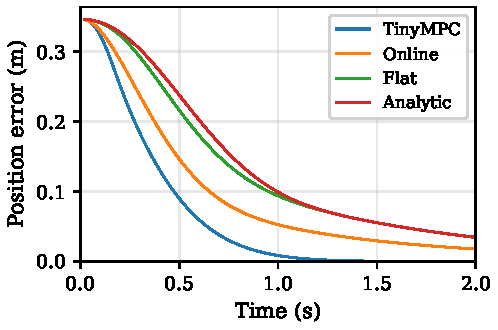
\includegraphics[width=\columnwidth]{figures/fig_hover.pdf}
  \caption{Hover stabilization: position error over time for all
    four variants. Initial displacement $(0.2, 0.2, -0.2)$\,m.
    All variants converge; the flat-parameterized controllers
    trade slightly slower convergence for significantly lower
    computation per step.}
  \label{fig:hover}
\end{figure}

\subsection{Figure-Eight Trajectory Tracking}

The reference is a figure-eight in the $xz$-plane with amplitude 0.5\,m
and period 3.7\,s.
Horizon $N=15$, penalty $\rho = 5$, $N_{\mathrm{sim}} = 200$ steps.
The Flat Template uses 21 cache entries sampled uniformly over one period.

\begin{table}[t]
\centering
\caption{Figure-eight trajectory tracking ($N_{\mathrm{sim}}=200$, $\rho=5$, $N=15$).}
\label{tab:traj}
\begin{tabular}{@{}lcccc@{}}
\toprule
 & Tiny & Online & Flat & Analytic \\
 & MPC & Relin & Template & Template \\
\midrule
Avg.\ pos.\ error (m)  & \textbf{0.033} & 0.035 & 0.035 & 0.036 \\
Max pos.\ error (m)    & \textbf{0.091} & 0.092 & 0.113 & 0.116 \\
Avg.\ ADMM iters       & 8.0 & 5.1 & 3.6 & 0 \\
Total ADMM iters       & 1598 & 1023 & 714 & 0 \\
Wall time (s)          & 1.16 & 22.02 & 0.75 & \textbf{0.26} \\
\bottomrule
\end{tabular}
\end{table}

\begin{figure}[t]
  \centering
  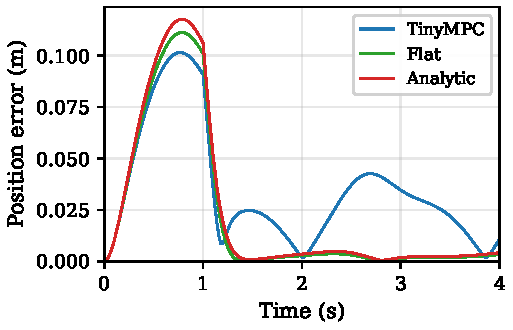
\includegraphics[width=\columnwidth]{figures/fig_traj_error.pdf}
  \caption{Figure-eight tracking: position error over time.
    All variants achieve comparable accuracy;
    the periodic structure reflects the trajectory curvature.}
  \label{fig:traj_error}
\end{figure}

\begin{figure}[t]
  \centering
  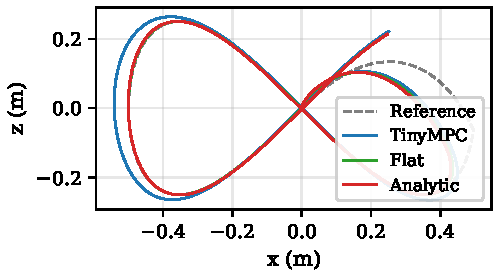
\includegraphics[width=\columnwidth]{figures/fig_traj_xz.pdf}
  \caption{Figure-eight tracking: $x$--$z$ plane view.
    The Flat Template and Analytic Template closely follow
    the reference trajectory (dashed), comparable to TinyMPC.}
  \label{fig:traj_xz}
\end{figure}

On the figure-eight trajectory (Table~\ref{tab:traj},
Figs.~\ref{fig:traj_error}--\ref{fig:traj_xz}),
all four variants
achieve similar average tracking errors ($0.033$--$0.036$\,m),
demonstrating that the flat-parameterized linearization is sufficiently
accurate for moderate-aggressiveness trajectories.
The key differences are computational:
\begin{itemize}
  \item The Flat Template requires $55\%$ fewer total ADMM iterations
    than TinyMPC and runs $1.5\times$ faster in wall-clock time.
  \item Online relinearization is $29\times$ slower than the
    Flat Template due to per-step autograd Jacobian evaluation and
    DARE solves, despite using fewer ADMM iterations.
  \item The Analytic Template achieves $4.5\times$ speedup over
    TinyMPC with only 0.003\,m additional average error, using
    \emph{zero} ADMM iterations.
\end{itemize}

\subsection{Numerical Validation}

We verify the implementation with four tests:
\begin{enumerate}
  \item \textbf{Linearization consistency}: At hover,
    the analytic $A_d, B_d$ match the autograd-based Jacobians
    to within $10^{-3}$ in position-velocity coupling and
    $10^{-15}$ in torque allocation.
    Attitude-related entries differ by ${\sim}2\times$ due to
    the Euler-angle vs.\ quaternion-error parameterization.
  \item \textbf{Gain approximation}: Over 100 random $\balpha$ samples
    with $\|a\| \leq 3$\,m/s$^2$,
    the first-order gain approximation~\eqref{eq:K_interp}
    achieves mean relative Frobenius error of 4\%.
  \item \textbf{Control equivalence}: At hover with inactive
    constraints, the Analytic Template output equals
    the 1-iteration Flat Template output to machine precision
    ($< 10^{-8}$).
  \item \textbf{Flat equilibrium}: For 20 random $\balpha$ values,
    $f(x^*(\balpha), u^*(\balpha))$ produces the expected
    continuous-time derivatives to $< 10^{-14}$.
\end{enumerate}

% ================================================================
\section{Discussion}\label{sec:discussion}

\textbf{When does the fixed linearization suffice?}
For near-hover operation, TinyMPC's fixed linearization is optimal
by construction.
The flat-parameterized variants become advantageous when the trajectory
induces significant attitude variation---the equilibrium shift
ensures the ADMM solver operates near zero error at every timestep,
improving convergence.

\textbf{Computational hierarchy.}
The five variants form a hierarchy of decreasing online cost
(see also the equivalence chain~\eqref{eq:full_chain}):
\begin{center}
\small
\begin{tabular}{@{}lcccc@{}}
\toprule
Variant & Online ops & Constr. & Conv. & Sched. \\
\midrule
Online Relin & $O(n^3) {+} K O(n^2)$ & Hard & Lin. & $\R^n$ \\
Flat Template & $K \cdot O(n^2)$ & Hard & Lin. & $\R^4$ \\
Barrier + IPM & $K_{\text{I}} \cdot O(n^2)$ & Hard & Quad. & $\R^4$ \\
Barrier & $O(n \cdot m)$ & Soft & --- & $\R^4$ \\
Analytic & $O(n \cdot m)$ & Clip & --- & $\R^4$ \\
\bottomrule
\end{tabular}
\end{center}
The Flat Template has the same per-iteration cost as TinyMPC but
converges in fewer iterations due to better-conditioned linearization.
The Barrier Template (Section~\ref{sec:barrier}) provides soft
constraint satisfaction at the same ${\sim}260$-operation cost as
the Analytic Template, by absorbing log-barrier information into
the DARE cache.
With optional IPM refinement (2--3 Newton steps),
it achieves hard constraint satisfaction with quadratic convergence---fewer
iterations than ADMM for the same accuracy.
The Analytic Template ($\mu = 0$) trades all constraint handling
for extreme efficiency.

\textbf{What is new vs.\ what is classical.}
The individual mathematical ingredients---differential
flatness~\cite{fliess1995,mellinger2011},
gain scheduling~\cite{rugh2000},
and Riccati sensitivity~\cite{hewer1971,konstantinov1993}---are
well established.
Our contribution is their specific combination in the context
of embedded ADMM-based MPC:
(i)~using flatness to compress the scheduling dimension from
$n$ to~4,
(ii)~caching the \emph{augmented} DARE (with ADMM penalty $\rho$)
rather than the standard LQR DARE,
(iii)~showing the equivalence between the zero-iteration ADMM
forward pass and the flat gain schedule,
and (iv)~absorbing log-barrier constraint penalties into the DARE
cache so that the zero-iteration controller is inherently
constraint-aware (Section~\ref{sec:barrier}).
This combination yields the 240-float, 260-operation
datapath of the Analytic Template---a level of compactness
not achievable by generic gain scheduling or LPV approaches
without the flatness reduction---while the barrier augmentation
adds constraint awareness at no additional online cost.

\textbf{FPGA portability.}
The analytic linearization (Section~\ref{sec:linearize}) and the
Analytic Template (Section~\ref{sec:analytic}) are composed entirely
of elementary operations: trigonometric functions, multiplications,
and additions.
There are no loops with data-dependent iteration counts
and no matrix inversions.
The 240-float storage and ${\sim}260$-operation datapath
are directly realizable as a fixed-function pipeline.

\textbf{Limitations.}
The first-order gain approximation~\eqref{eq:K_interp} degrades
for large $\|\balpha - \balpha_0\|$.
For highly aggressive maneuvers, the Flat Template MPC with a
sufficiently dense cache grid is preferred.
The current Python results do not reflect embedded timing;
C/C++ implementation with Crazyflie hardware experiments
is ongoing work.

% ================================================================
\section{Conclusion}\label{sec:conclusion}

We presented three extensions of TinyMPC that exploit differential
flatness to adapt the linearization point along a trajectory.
The Flat Template MPC precomputes a family of DARE caches indexed
by the flat parameter $\balpha$, preserving TinyMPC's
matrix-inversion-free online structure while achieving
faster ADMM convergence.
The Analytic Template further reduces the online computation
to ${\sim}260$ arithmetic operations by replacing ADMM
with a first-order gain interpolation.
The Barrier-Augmented Template absorbs log-barrier constraint
penalties into the DARE cache, providing inherent constraint
awareness at zero additional online cost, with optional
Newton--IPM refinement for hard constraint satisfaction
at quadratic convergence.
Preliminary simulation results demonstrate that
the flat-parameterized variants
maintain tracking accuracy comparable to online relinearization
at substantially lower computational cost.
Future work includes C implementation targeting the
Crazyflie 2.1 STM32F405 microcontroller,
FPGA synthesis of the Analytic Template datapath,
numerical validation of the Barrier-Augmented Template,
and extension to wind-disturbance rejection.

% ================================================================
\bibliographystyle{IEEEtran}
\begin{thebibliography}{10}

\bibitem{tinympc}
A.~Alavilli, K.~Nguyen, S.~Schoedel, B.~Plancher, and Z.~Manchester,
``TinyMPC: Model-predictive control on resource-constrained
microcontrollers,''
in \emph{Proc.\ IEEE Int.\ Conf.\ Robotics and Automation (ICRA)},
2024.

\bibitem{mellinger2011}
D.~Mellinger and V.~Kumar,
``Minimum snap trajectory generation and control for quadrotors,''
in \emph{Proc.\ IEEE Int.\ Conf.\ Robotics and Automation (ICRA)},
2011, pp.~2520--2525.

\bibitem{murray1995}
R.~M.~Murray, M.~Rathinam, and W.~Sluis,
``Differential flatness of mechanical control systems: A catalog of
prototype systems,''
in \emph{Proc.\ ASME Int.\ Mechanical Engineering Congress},
1995.

\bibitem{mueller2015}
M.~W.~Mueller, M.~Hehn, and R.~D'Andrea,
``A computationally efficient motion primitive for quadrocopter
trajectory generation,''
\emph{IEEE Trans.\ Robotics}, vol.~31, no.~6, pp.~1294--1310, 2015.

\bibitem{fliess1995}
M.~Fliess, J.~L{\'e}vine, P.~Martin, and P.~Rouchon,
``Flatness and defect of non-linear systems: introductory theory
and examples,''
\emph{Int.\ J.\ Control}, vol.~61, no.~6, pp.~1327--1361, 1995.

\bibitem{osqp}
B.~Stellato, G.~Banjac, P.~Goulart, A.~Bemporad, and S.~Boyd,
``OSQP: An operator splitting solver for quadratic programs,''
\emph{Mathematical Programming Computation}, vol.~12, pp.~637--672,
2020.

\bibitem{boyd2011}
S.~Boyd, N.~Parikh, E.~Chu, B.~Peleato, and J.~Eckstein,
``Distributed optimization and statistical learning via the alternating
direction method of multipliers,''
\emph{Foundations and Trends in Machine Learning}, vol.~3, no.~1,
pp.~1--122, 2011.

\bibitem{faessler2018}
M.~Faessler, A.~Franchi, and D.~Scaramuzza,
``Differential flatness of quadrotor dynamics subject to rotor drag
for accurate tracking of high-speed trajectories,''
\emph{IEEE Robotics and Automation Letters}, vol.~3, no.~2,
pp.~620--626, 2018.

\bibitem{rugh2000}
W.~J.~Rugh and J.~S.~Shamma,
``Research on gain scheduling,''
\emph{Automatica}, vol.~36, no.~10, pp.~1401--1425, 2000.

\bibitem{shamma1991}
J.~S.~Shamma and M.~Athans,
``Guaranteed properties of gain scheduled control for linear
parameter-varying plants,''
\emph{Automatica}, vol.~27, no.~3, pp.~559--564, 1991.

\bibitem{hewer1971}
G.~A.~Hewer,
``An iterative technique for the computation of the steady state
gains for the discrete optimal regulator,''
\emph{IEEE Trans.\ Automatic Control}, vol.~16, no.~4,
pp.~382--384, 1971.

\bibitem{konstantinov1993}
M.~M.~Konstantinov, P.~Hr.~Petkov, and N.~D.~Christov,
``Perturbation analysis of the discrete Riccati equation,''
\emph{Kybernetika}, vol.~29, no.~1, pp.~18--29, 1993.

\bibitem{bemporad2002}
A.~Bemporad, M.~Morari, V.~Dua, and E.~N.~Pistikopoulos,
``The explicit linear quadratic regulator for constrained systems,''
\emph{Automatica}, vol.~38, no.~1, pp.~3--20, 2002.

\bibitem{boyd2004}
S.~Boyd and L.~Vandenberghe,
\emph{Convex Optimization}.
Cambridge Univ.\ Press, 2004.

\bibitem{jordana2023}
A.~Jordana, S.~Kleff, A.~Meduri, J.~Carpentier, N.~Mansard,
and L.~Righetti,
``Stagewise implementations of sequential quadratic programming
for model-predictive control,''
in \emph{Proc.\ IEEE/RSJ IROS}, 2023.

\end{thebibliography}

\end{document}
